\Author{\daAuthorOne}
% \usepackage[backend=biber, style=alphabetic]{biblatex}

The Admin Panel is an administrative control center to efficiently manage all addresses within a single environment. It is used for planning upcoming "Sternsinger" events, ensuring that all required addresses are covered and effectively distributed among participating groups. Additionally, it provides a way to assign areas containing addresses that a group needs to visit. This zoning feature ensures that each group is responsible for only the addresses within their designated area.\blankLine

This tool enables authorized users to perform CRUD operations (Create, Read, Update, Delete) on addresses, streets, and areas. These features make it easy to address issues quickly and make changes to the areas that participants need to visit. For example, when a new street is added to the neighborhood, the administrator can update the system to include it and assign it to the appropriate area. Similarly, if a group withdraws from the event, the administrator can reassign any unvisited addresses to other groups. This ensures that the data remains up-to-date, allowing quick reactions to special cases, helping with the planning and execution of "Sternsinger" events.\blankLine

This chapter will outline the implementation of the Admin Panel, detailing its components, functionalities, and widgets, and providing guidance on how to use them.\blankLine\blankLine


\subsection{Navigation}

\begin{figure}[H]

\begin{minipage}{0.58\textwidth}
    \setstretch{1.5} % Erhöht den Zeilenabstand
    To navigate between pages, a sidebar on the left is used, which can be toggled with a button in the top-left corner of the page. It displays a list of all pages, allowing users to switch between them with a click.

    The navigation is implemented in the \texttt{AdminNavigation} component. The menu contains a list of \texttt{ScreenItems} (see \ref{fig:ScreenItem}), which store the title with the corresponding page. These titles are displayed at the top of the screen above the page. To keep track of the currently selected page, an internal state (\texttt{indexState}) is used. Whenever a page is selected in the sidebar, the \texttt{indexState} is updated, and the corresponding page is displayed. This widget is the main component. It ensures that all pages are properly displayed.

    \end{minipage}
    \hfill
    \begin{minipage}{0.38\textwidth}
    \centering
    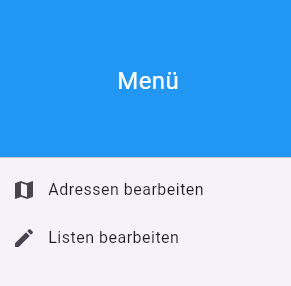
\includegraphics[width=\linewidth]{images/AdminPanel/Menu.png}
    \caption{Navigation in Admin Panel}
    \label{fig:adminpanel_navigation}
\end{minipage}

\end{figure}



\begin{subsection}{AddressPage}
    \sloppy
    The first page, called \texttt{AddressPage} provides an interface for managing address data, including creation, modification, and deletion. It uses a form with various input fields and a visualization component that displays addresses on a map or in a database view. The layout is divided into two parts:

    \begin{itemize}
        \item On the right side, all addresses are shown in either the \texttt{AdminMapComponent} (\ref{fig:AdminMapComponent}), displaying addresses on a map, or the \texttt{DatabaseViewComponent} (\ref{fig:DatabaseViewComponent}), showing them in a table.
        \item On the left side of the page, there are \texttt{InputFields} (\ref{fig:InputField}), which are used to enter new information about a new address or edit existing ones.
    \end{itemize}

    \newpage

    The following elements overlay the \texttt{AdminMapComponent}:

    \begin{itemize}
        \item A field to filter the addresses that are displayed.
        \item A button with a dropdown menu to select and edit a street.
        \item A switch to toggle between the \texttt{AdminMapComponent} and the \texttt{DatabaseViewComponent}.
        \item An information box in the bottom left corner to display \texttt{Notifications} (\ref{fig:Notification}) about the completed operations.
        \item A field in the bottom right corner to display the coordinates of the mouse pointer on the map.
    \end{itemize}
    

    \begin{figure}[H]
        \centering
        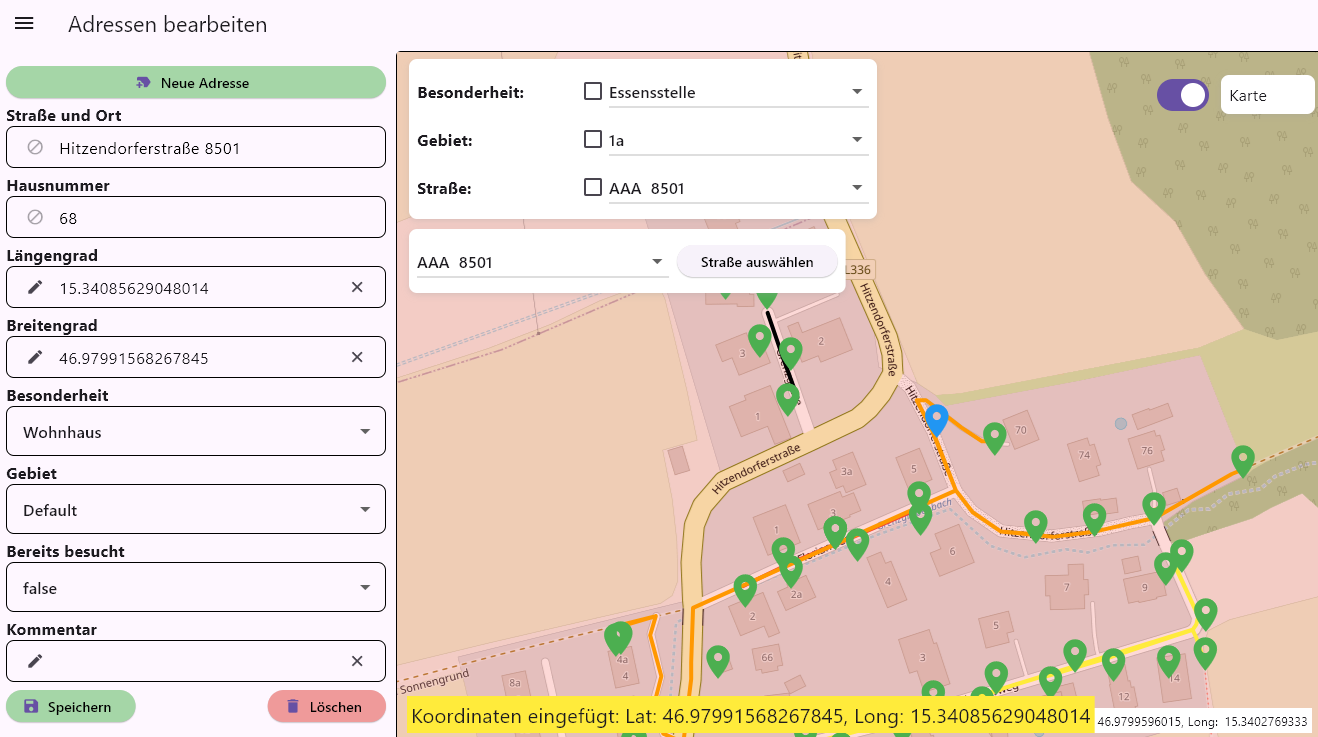
\includegraphics[width=1\linewidth]{images/AdminPanel/AddressPage.png}
        \caption{AddressPage}
    \end{figure}
\end{subsection}

\newpage

\subsubsection{Add Address}
    \label{fig:Add Address}

    \sloppy
    To add a new address, the "Neue Adresse" button is pressed. This triggers the \texttt{onClickNewAddress} method, which performs several key operations:  

    \begin{itemize}  
        \item All \texttt{InputFields} are cleared.  
        \item The boolean variable \texttt{isNewAddress} is set to \texttt{true}, indicating that a new address is being created.  
    \end{itemize}  
    
    The cleared fields can then be filled with the new information. When the "Speichern" button is pressed, the \texttt{saveAddress} method is called. This method performs several validation checks, as shown in \ref{fig:Validation}. If the address is valid, the \texttt{AdminAddressProvider} adds it to the database, a \texttt{notification} is displayed, and the newly added address appears.\blankLine
    
    When the map is clicked, the \texttt{onClickNewAddress} method is also invoked within the \texttt{AdminMapComponent}. The method receives the click coordinates as parameters to create the address at the selected location.  
    

\subsubsection{Edit Address}
\sloppy % Damit der Text (\texttt{DatabaseViewComponent}) nicht über den Rand hinausragt
Existing addresses can be edited by selecting them in either the \texttt{AdminMapComponent} or the \texttt{DatabaseViewComponent}.
The selection fills the \texttt{InputFields} with the information of the address, and in this case, the boolean variable \texttt{isNewAddress} is set to \texttt{false} to indicate that an existing address is being updated.\blankLine

\sloppy
The administrator can then edit the information and press the "Speichern" button. This triggers the \texttt{saveAddress} method, which performs the same validation checks as when adding a new address. The \texttt{AdminAddressProvider} updates the selected address in the database, and the \texttt{notification} is displayed. \newpage

\subsubsection{Delete Address}
After selecting an address, the administrator can press the "Löschen" button to delete it. This triggers the \texttt{deleteAddress} method, which calls the \texttt{AdminAddressProvider} to delete the selected addresses.\blankLine

The method also triggers the \texttt{showDeleteDialog} method, which displays an \texttt{AlertDialog} to confirm the action and prevent accidental deletions.

\begin{figure}[H]
    \centering
    
\includegraphics[width=0.6\linewidth]{images/AdminPanel/DeleteDialog.png}
    \caption{Dialog to confirm deletion}
\end{figure}

\subsubsection{Validation}
\label{fig:Validation}
    Validation is the process of checking that data meets specific criteria before it is accepted and added to a system or database. This ensures that the data is accurate, consistent, and conforms to required standards. Validation prevents errors and inconsistencies that could arise from invalid or incomplete data, maintaining the integrity and reliability of the system. It helps catch mistakes early, such as missing fields or incorrect data inputs. By ensuring that only valid data is processed, validation plays a crucial role in preserving data quality. \autocite{ContributorstoWikimediaprojects2025Feb}

\paragraph{isDuplicateAddress}
    To determine whether an edited or newly added address already exists in the system, the new address is compared against all existing addresses to detect potential duplicates before the address is saved. The comparison takes place within the \texttt{saveAddress} method, which handles the saving operation. If an address is found to be identical to an existing one, the method returns \texttt{true}, indicating that the address is a duplicate. If no match is found, it returns \texttt{false}, confirming that the address is unique and can be safely added to the database.\blankLine

    A duplicate address is identified by the following criteria:\blankLine
    \textbf{street name, postal code, and house number}
    


\newpage

\paragraph{InputField filled Validation}
To verify that all required \texttt{InputFields} are properly filled, the \texttt{validateAddressFields} method is called.

To start the process, a new \texttt{Address} object is created and passed to the \texttt{validateAddressFields} method. The method checks each field within the \texttt{Address}. If a field is missing or incomplete, a \texttt{notification} (see \ref{fig:Notification}) is displayed to inform the user of the missing data, such as "Strasse fehlt" or "Koordinaten fehlen." If all fields are correctly filled out, the method returns \texttt{true}, signaling that the address can be saved. However, if any field is incomplete, the method returns \texttt{false}, preventing the address from being saved until all required information is provided.



\paragraph{InputField Coordinates Validation}
\label{fig:InputField Coordinates Validation}
    The \texttt{InputField} validates \textbf{latitude} and \textbf{longitude} inputs, ensuring correct coordinates. Validation is applied only when the \texttt{isCoordinateInput} parameter is set to \texttt{true}. In that case, the \texttt{inputFormatter} is passed to the \texttt{textfield}. This \texttt{inputFormatter} guarantees that only valid inputs are accepted. These are the three validators used:


    \begin{itemize}
        \item A \texttt{FilteringTextInputFormatter} with a regular expression is used to restrict the input to digits, decimal points, and an optional minus sign at the beginning.
        \begin{figure}[H]
            \centering
            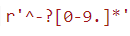
\includegraphics[width=0.2\linewidth]{images/AdminPanel/regexInputFormatter.png}
            \caption{Regular expression for input validation}
        \end{figure}
        \item A \texttt{TextInputFormatter} prevents multiple decimal points in a single number. If a user attempts to insert a second decimal point, the input is automatically rejected.
        \item The final \texttt{TextInputFormatter} ensures that the number of digits before the decimal point is limited to a maximum of 3 and the value itself does not exceed 180.
    \end{itemize}
    
\newpage


\subsubsection{Additional Functionalities}
    This section outlines several functionalities that have been integrated to improve the overall usability of the application. These enhancements are specifically designed to simplify tasks while ensuring an intuitive user experience.

\paragraph{Notification}
\label{fig:Notification}

    To notify the administrator about the success or failure of an operation, a \texttt{notification} is displayed at the bottom left, overlaying the \texttt{AdminMapComponent}. This \texttt{notification} appears when:

    \begin{itemize}
        \item An address has been added, edited, or deleted.
        \item Validation has failed.
        \item Coordinates are selected on the \texttt{AdminMapComponent} (\ref{fig:Select Coordinates on Map}).
    \end{itemize}


\begin{figure}[H]
    \centering
    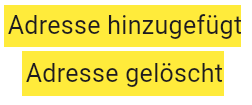
\includegraphics[width=0.4\linewidth]{images/AdminPanel/NotificationExamples.png}
    \caption{Notification examples}
\end{figure}

To display this notification, the \texttt{showNotification} method is called. This method sets the \texttt{notificationVisible} variable to \texttt{true} and starts a \texttt{timer} to reset it to \texttt{false} after three seconds, causing the notification to disappear shortly after. The method accepts a message as a parameter, which is stored in the \texttt{notificationText} variable. When the \texttt{notificationVisible} variable is set to \texttt{true}, the UI component that shows the notification is rendered.


\subsubsection{Edit multiple Addresses}
\label{fig:Edit multiple addresses}
To make it easier to edit multiple addresses at once, the control|command key on the keyboard is listened to, meaning the system detects and responds to when the key is pressed. When this key is pressed, the \texttt{isCtrlPressed} variable is set to \texttt{true}. This variable is passed to the \texttt{DatabaseViewComponent} and the \texttt{AdminMapComponent} to inform them that multiple addresses are to be selected.\blankLine


To detect when the control|command key is pressed or released, the predefined \texttt{RawKeyboardListener} widget is used. This widget listens for keyboard events and updates the state of the \texttt{isCtrlPressed} variable accordingly. When the key is pressed, the widget sets \texttt{isCtrlPressed} to \texttt{true}, indicating that it is being held down. Alternatively, when the  key is released, \texttt{isCtrlPressed} is set to \texttt{false}, signaling that the key is no longer pressed.

To handle repeated key presses effectively, especially when the CTRL key is held down, a condition is implemented to prevent continuously setting \texttt{isCtrlPressed} to \texttt{true}. This is achieved by checking the \texttt{event.repeat} property, ensuring that the variable is only updated when \texttt{event.repeat} is false.


The \texttt{markerSelected} method also updates the \texttt{InputField} by listing all house numbers of the selected addresses. This ensures that the user is presented with a clear overview of all the selected addresses, making it easier to manage multiple selections.

The \texttt{InputField} looks like this:
\begin{figure}[H]
    \centering
    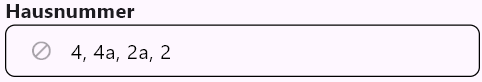
\includegraphics[width=0.6\linewidth]{images/AdminPanel/listedHouseNumbersInputField.png}
    \caption{House numbers of multiple selected Addresses}
\end{figure}

The selected addresses are saved in the \texttt{selectedAddresses} variable in the \texttt{AddressPage}. If multiple addresses are selected, certain \texttt{InputFields}, such as house numbers, coordinates, or comments, are disabled, as changing them for all selected addresses would not make sense. This is achieved by setting the \texttt{editable} parameter of these \texttt{InputFields} to \texttt{selectedAddresses.length <= 1}, ensuring that they are only editable when a single address is selected.


\subsubsection{Edit all Addresses from a Street}
All addresses on a street can be edited at once, simplifying bulk modifications. This process is similar to editing multiple addresses (\ref{fig:Edit multiple addresses}), but instead of manually selecting each address, the entire street is selected at once. This allows for quicker adjustments, ensuring consistency across all addresses on the selected street. Once a street is chosen, all associated addresses are automatically included in the selection. \blankLine

A street can be selected in two ways:  




\paragraph{Select a Street via AdminMapComponent}
Every click on the \texttt{AdminMapComponent} is checked to see if it is near a street. Since there is no predefined method to check if a point is on a street, the \texttt{isPointNearPolyline} method was implemented. This method checks whether the click was on the street. More information about this method can be found in the \texttt{AdminMapComponent} section \ref{fig:AdminMapComponent}.\

\begin{figure}[H]
    \centering
    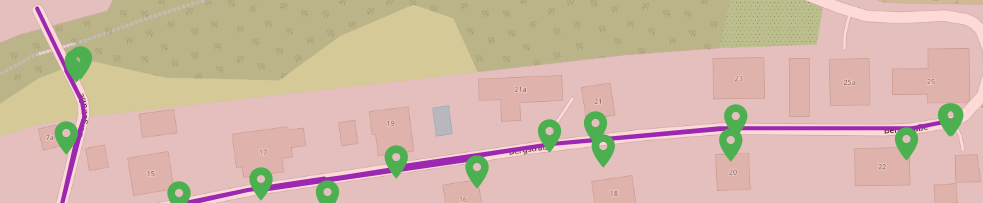
\includegraphics[width=0.6\linewidth]{images/AdminPanel/Street.png}
    \caption{Street visualization example in AdminMapComponent}
\end{figure}


\paragraph{Select a Street via Button}
This was implemented because selecting the street directly on the map could be a bit spotty in its working. Through this feature, a reliable way to select a street was available, even though in the final deployment, the street selection via map worked flawlessly. 
\begin{figure}[H]
    \centering
    \includegraphics[width=0.6\linewidth]{images/AdminPanel/SelectStreetButton.png}
    \caption{Field to select a Street}
\end{figure}

\newpage


\subsubsection{Edit Odd / Even Streets}
One requirement was that addresses from a street could be automatically assigned to two areas based on whether the house number is even or odd. This is because it is common for addresses with even house numbers to be on one side of the street and those with odd house numbers on the other side. This division makes it easier to assign the street sides to different areas so that "Sternsinger" participants don't have to cross the street as often.\blankLine 
To make this possible, the administrator first selects a street in the \texttt{AdminMapComponent} (\ref{fig:Select Street}), and then a blue button appears beneath the \texttt{InputFields}.
\begin{figure}[H]
    \centering
    
\includegraphics[width=0.6\linewidth]{images/AdminPanel/splitStreetButton.png}
    \caption{Button to split Street}
\end{figure}

\begin{figure}[H] 
    \begin{minipage}{0.6\textwidth}
        After pressing this button, a dialog appears, where the administrator can select the areas for addresses with even and odd house numbers on this street. The "Speichern" button triggers the \texttt{AdminAddressProvider} and displays a \texttt{notification} (\ref{fig:Notification}) indicating whether the operation was successful or not. Afterward, the dialog is closed.
    \end{minipage}
    \hfill
    \begin{minipage}{0.35\textwidth}
        \centering
        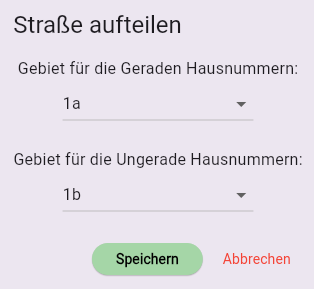
\includegraphics[width=\linewidth]{images/AdminPanel/splitStreetDialog.png}
        \caption{Dialog to split street}
    \end{minipage}
\end{figure}



\begin{figure}[H]
    \setstretch{1.5} % Erhöht den Zeilenabstand
    \centering
    \begin{minipage}{0.55\textwidth} % Linke Seite für den Text
        \subsubsection{Filter}
        With the Filter field, the administrator can filter the addresses displayed. It contains three dropdown menus to set the filter criteria, with one checkbox for each to toggle them. These filters can be combined as desired. 
    \end{minipage}
    \hfill 
    \begin{minipage}{0.4\textwidth} % Rechte Seite für das Bild
        \centering
        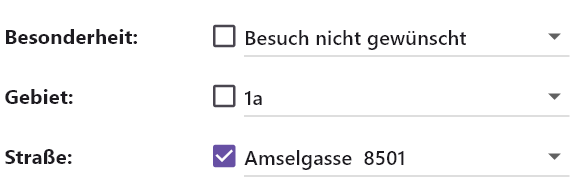
\includegraphics[width=\linewidth]{images/AdminPanel/FilterField.png}
        \caption{Filter in AddressPage}
        \label{fig:adminpanel_filter}
    \end{minipage}
\end{figure}

\newpage

The filter is passed and applied to both the \texttt{AdminMapComponent} and the \texttt{DatabaseViewComponent}. The criteria and their enabled/disabled state are managed by a series of variables within the \texttt{AddressPage} class. These variables control which filters are active and store the selected filter values. They are defined as follows:\blankLine

The filter is then applied to the addresses within the components. The filtering process is done step-by-step, starting with the area filter, followed by the special feature filter, and finally the street filter. If any of the filter conditions are met, the addresses are filtered accordingly. Only the \texttt{filteredAddresses} are displayed in the \texttt{AdminMapComponent} and the \texttt{DatabaseViewComponent}.
 

\subsection{ListEditPage}
The \texttt{ListEditPage} is used to manage \textbf{streets}, \textbf{special features}, and \textbf{areas}. It allows the administrator to add, edit, and delete these entities. The page is divided into two sections. On the right side, all entities are displayed in a table and can be selected. On the left, there is a dropdown menu for selecting between the three options. The information of the selected item is shown in \texttt{InputFields}, where it can be edited, saved, or deleted using the "Speichern" or "Löschen" button.

\begin{figure}[H]
    \centering
    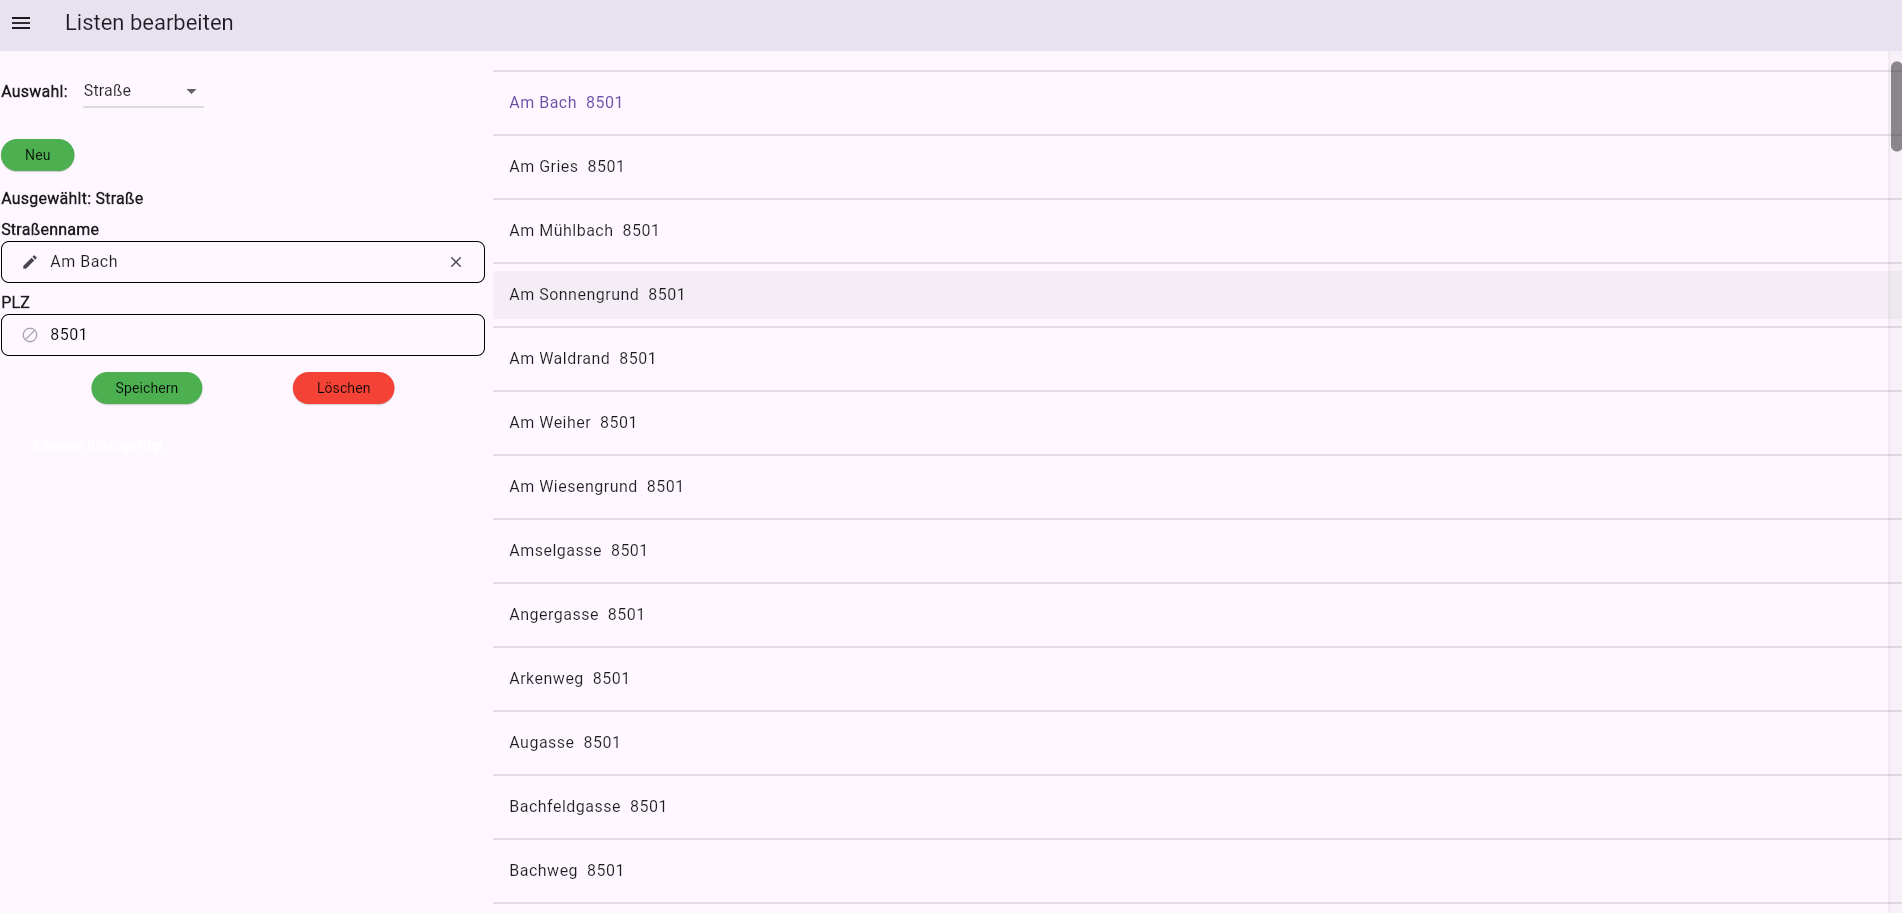
\includegraphics[width=0.9\linewidth]{images/AdminPanel/ListEditPage.png}
    \caption{ListEditPage}
\end{figure}

\subsubsection{QR-Code Visualization for Areas}
To make it easier for users of the user application to access information about their area, a QR-Code is generated for the selected area, which can be scanned to get all information. The QR-Code contains the name of the area. The currently selected area is saved in the \texttt{selectedItem} variable. To display the QR-Code, the predefined \texttt{QrImageView} is used.

\begin{figure}[H]
    \centering
    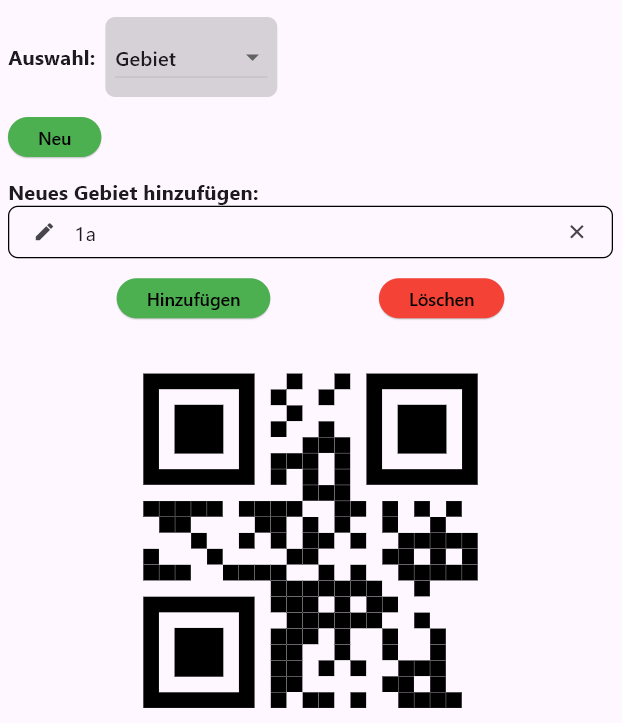
\includegraphics[width=0.4\linewidth]{images/AdminPanel/QrImageView.png}
    \caption{QR-Code for Area}
\end{figure}

\subsubsection{QR-Code-PDF Download}
A PDF containing  QR-codes for all areas can be downloaded, making it easier to distribute the information to users. The PDF is generated using the \texttt{savePDF} method of the \texttt{PDFSaver} class.\blankLine

To generate the QR-codes, the \texttt{generateQRCode} method in the \texttt{ListEditPage} class is used. This method takes a \texttt{String} as a parameter and converts it into a QR-code using the predefined \texttt{QrPainter}, which helps in rendering it \autocite{pub.dev/QrPainter-class}. It then generates an image of the QR-code, converts it into PNG byte data, and transforms the byte data into a list of bytes (\texttt{Uint8List}) to be used in the PDF. \blankLine

Then, the \texttt{savePdf} method of the \texttt{PDFSaver} class creates a PDF document containing the QR-codes for all areas. It uses the predefined \texttt{pdf} package (imported as \texttt{pw}) to manage the PDF document \autocite{pub.dev/pdf}. The function starts by initializing a new PDF using the \texttt{pw.Document()} class and an empty list to store the generated QR-codes. The method then iterates over the list of areas, generating a code for each description of all areas using \texttt{generateQRCode} and adding it to the list.\blankLine

Afterward, a page is added to the PDF document using the \texttt{pw.MultiPage} widget. This page includes a title and the description of each area along with its corresponding QR-code. Once the page content is built, the PDF data is saved by calling \texttt{pdf.save()}. Finally, the \texttt{PdfSaver.savePdf} method is called to save the PDF as "Gebiete.pdf."

\begin{figure}[H]
    \centering
    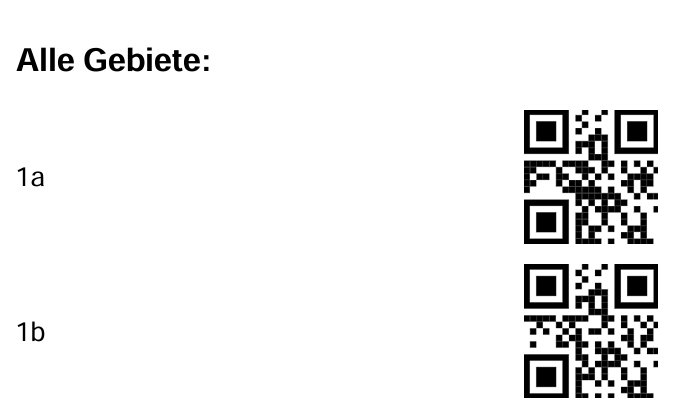
\includegraphics[width=0.5\linewidth]{images/AdminPanel/GebietePDF.png}
    \caption{PDF with QR-Codes for all Areas}
\end{figure}


\subsubsection{Icon for Special Features}
\begin{figure}[H] 
    \begin{minipage}{0.6\textwidth}
        When a special feature is selected, an icon is displayed to visually represent it. The administrator has the option to upload a custom image to use as the icon for the selected special feature. Once the image is uploaded and the "Speicher" button is pressed, it is saved in the database and used as the icon, allowing for easy visual identification of the special feature. This icon is displayed in the user application.
    \end{minipage}
    \hfill
    \begin{minipage}{0.35\textwidth}
        \centering
        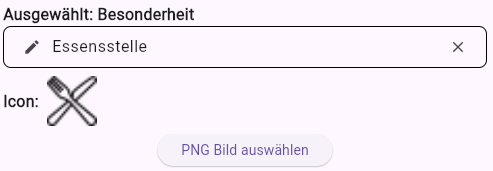
\includegraphics[width=\linewidth]{images/AdminPanel/chooseIcon.png}
        \caption{choose Icon for Special Feature}
    \end{minipage}
\end{figure}

\newpage

\subsection{Components}
Components play a key role in structuring the Admin Panel. Each one is designed to handle specific tasks or display certain UI elements, making them reusable throughout the application. 
\subsubsection{AdminMapComponent}
\label{fig:AdminMapComponent}
This component displays the addresses on a geographic map. The map used is OpenStreetMap, which is free to use for everyone. Although the Admin Panel is not used commercially, OpenStreetMap's attribution rules are followed. The map shows the required copyright notice "© OpenStreetMap contributors" in the bottom-left corner. The word "OpenStreetMap" is clickable and links directly to \url{https://www.openstreetmap.org/copyright}, opening the official license page in a new tab. This meets OpenStreetMap's license requirements by clearly acknowledging the data source and linking to their terms. \autocite{OpenStreetMap}

\begin{figure}[H]
    \centering
    
\includegraphics[width=0.2\linewidth]{images/AdminPanel/Openstreetmapverweis.png}
    \caption{OpenStreetMap attribution}
\end{figure}




\paragraph{Select a Street}
\label{fig:Select Street}

To select a street, the \texttt{isPointNearPolyline} method was implemented. This method checks whether the click was on a street. It takes the coordinates of the click as a \texttt{LatLng} object and a street as a list of \texttt{LatLngs}. After each click on the map, a loop is triggered that calls the \texttt{isPointNearPolyline} method for every street, passing the click coordinates during each iteration.\blankLine

The \texttt{isPointNearPolyline} method uses another loop that iterates over all points of the street. Since the street is represented as a list of \texttt{LatLng} objects, each pair of consecutive points is connected to form a line segment. During each iteration of the loop, a helper method \texttt{isNear} is called to calculate the distance between the click and the currently iterated line segment.

\newpage

The \texttt{isNear} method takes the click point, the two points for the line and the tolerance. If the distance is smaller than the predefined tolerance, the method returns \texttt{true}, indicating that the click was on the street.\blankLine

The method uses the Manhattan distance to determine the distance between the click and the line. The Manhattan distance, also known as taxicab or city block distance, measures the distance between two points in a grid-based system. It is calculated as the sum of the absolute differences of the x- and y-coordinates.\blankLine
Why the absolutes? The absolute value ensures that the distance is always positive, regardless of the direction. If you were to walk 5 blocks north or 5 blocks south, the distance is the same. It's 5 blocks. This distance is then compared to the tolerance. \autocite{AlgoDaily2025Mar}

\begin{center}
    {\Large  $d_{\text{Manhattan}} = |x_2 - x_1| + |y_2 - y_1|$}
\end{center}

\lstset{style=mycsharp, caption=isNear method}
\begin{lstlisting}
bool _isNear(LatLng p, LatLng a, LatLng b, double tol) {
    double dx = b.latitude - a.latitude, dy = b.longitude - a.longitude;
    double t = ((p.latitude - a.latitude) * dx + (p.longitude - a.longitude) * dy) / (dx * dx + dy * dy);
    t = t.clamp(0, 1);
    return (p.latitude - (a.latitude + t * dx)).abs() + (p.longitude - (a.longitude + t * dy)).abs() <= tol;
}
\end{lstlisting}



\paragraph{Select Coordinates on Map}
\label{fig:Select Coordinates on Map}

To select coordinates to the currently selected address, a long press can be done on the map. The method \texttt{onCoordinateSelected} is then called via a callback from the \texttt{AdminMapComponent}. This sets the coordinates of the address to the coordinates of the click. The \texttt{InputFields} are then filled with the new coordinates.\

Because it would not make any sense to select coordinates for multiple addresses at once, the length of the \texttt{selectedAddresses} list is checked. Only if it is smaller than 2, the coordinates can be selected.


\subsubsection{DatabaseViewComponent}
\label{fig:DatabaseViewComponent}
To display the addresses in a table, this component was implemented. It takes the \texttt{selectedAddresses}, the filter variables, and the \texttt{isCtrlPressed} variable from the \texttt{AddressPage} as parameters. The \texttt{isCtrlPressed} variable is used to track whether multiple addresses are being selected. The \texttt{selectedAddresses} are shown in the table and can be selected by clicking on them.\blankLine

Above the table, two fields are displayed: one showing the number of selected addresses and the other showing the total number of found addresses. The table is implemented using the \texttt{ListView} widget, a predefined widget in Flutter.


\begin{figure}[H]
    \centering
    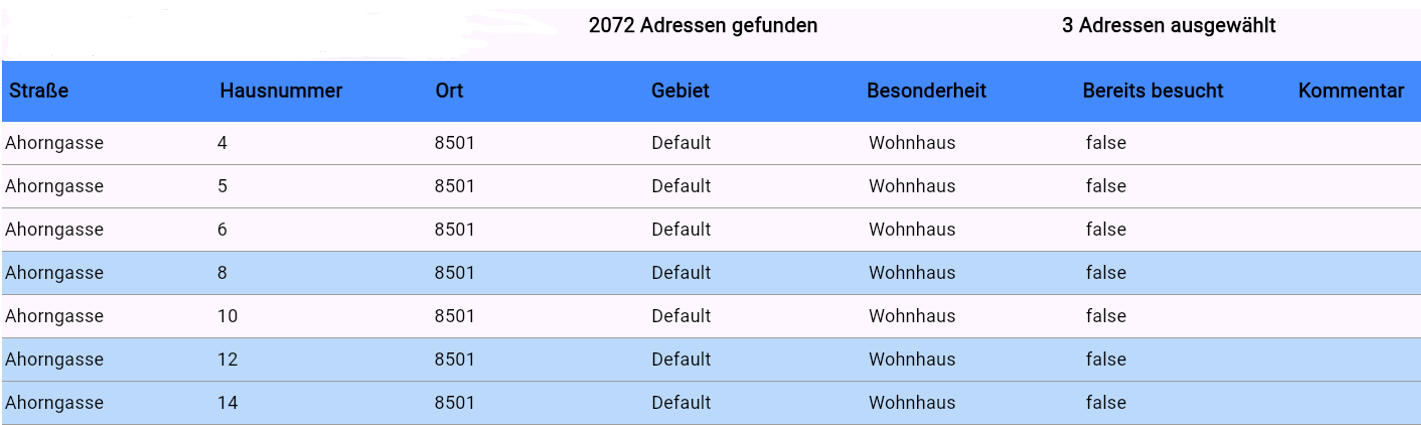
\includegraphics[width=0.9\linewidth]{images/AdminPanel/DataBaseViewComponent.png}
    \caption{DatabaseViewComponent}
\end{figure}


\subsubsection{PDFSaver}
The \texttt{PdfSaver} class provides functionality for saving PDF files from a byte array. The static method \texttt{savePdf} handles the saving process depending on the platform. \blankLine

For web applications, it creates a \texttt{Blob} containing the PDF data, generates a temporary URL, and triggers a download via an \texttt{AnchorElement}. After the download starts, the temporary URL is revoked to free resources.\blankLine

On non-web platforms, the method utilizes the \texttt{FileSaver} package to store the PDF file. The \texttt{saveFile} function is used, specifying the file name, byte data, and MIME type to ensure proper file handling.


\newpage
  \subsubsection{AdminAddressProvider}
  This class serves as a bridge between the Admin Panel and the backend. It is responsible for all CRUD operations on addresses, streets, special features, and areas. It is used in the \texttt{AddressPage} and the \texttt{ListEditPage}. \blankLine

  The \texttt{AdminAddressProvider} includes the \texttt{ChangeNotifier} mixin. A mixin is a way to reuse code across multiple classes without using inheritance, as in Java. \autocite{dart.dev} The \texttt{ChangeNotifier} mixin is used to notify the UI when the data changes. \autocite{flutter.dev}  \blankLine
  
  This notification is triggered by calling the \texttt{notifyListeners} method. Below is a typical method in the \texttt{AdminAddressProvider} class, which demonstrates these functionalities:  
  

\begin{itemize}
    \item \texttt{async}: enables non-blocking operations and ensures that the UI remains responsive while waiting for tasks like network requests to complete.
    \item \texttt{await http.get}: sends a GET request to the server to fetch all streets and waits for the response.
    \item \texttt{jsonDecode}: processes the JSON response from the server.
    \item \texttt{utf8.decode}: transforms the UTF-8 encoded response body into readable text.
    \item \texttt{map}: converts the decoded JSON to a list of \texttt{Street} objects.
    \item \texttt{sort}: sorts the list alphabetically.
    \item \texttt{notifyListeners}: notifies the listeners that the data has changed.
    \item \texttt{catch}: catches any errors that occur during the operation.
\end{itemize}

\subsection{Models}
Models represent and manage data structures within the Admin Panel. They are designed to encapsulate data and provide a structured approach for interacting with it. Various models have been developed to ensure maintainability and efficiency.



\subsubsection{AreaWithBorder}
To associate an area with its border coordinates, the \texttt{AreaWithBorder} model was introduced. It stores all border points as a list of \texttt{LatLng} objects, which are then used in the \texttt{AdminMapComponent} to draw the boundary. This visualization helps to clearly distinguish which addresses belong to which area.


\subsubsection{ScreenItem}
\label{fig:ScreenItem}
The \texttt{ScreenItem} was created to store data related to a menu option in the \texttt{AdminNavigation}. It is used to save the title, associated screen, and icon for each navigation item.

\subsection{Widgets}
Widgets are used to build and reuse UI components in Flutter. They help maintain a consistent look and feel across the entire interface, ensuring a seamless user experience. Several custom widgets were implemented for the Admin Panel.

\subsubsection{InputField}
\label{fig:InputField} 
This widget defines a customizable input field. The \texttt{InputField} requires a label and a \texttt{TextEditingController} to manage the input. Optional parameters include a boolean \texttt{editable}, a list of \texttt{Strings} called \texttt{dropDownOptions}, and a boolean \texttt{isCoordinateInput} to specify whether the input should be numeric.\blankLine

To indicate whether the \texttt{InputField} is editable, icons are displayed on the left side of the field. If the field is not editable, a blocked symbol appears. If it is editable, a pencil icon is shown. When the \texttt{InputField} is editable and not a dropdown, a cross icon appears on the right side. Pressing this icon clears the content.

\begin{figure}[H]
    \centering
    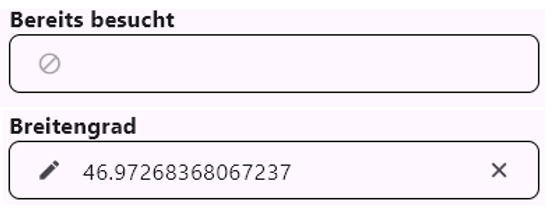
\includegraphics[width=0.4\linewidth]{images/AdminPanel/InputFieldExamples.png}
    \caption{InputField examples}
\end{figure}

If the \texttt{dropDownOptions} parameter is provided with a non-empty list of \texttt{Strings}, the input field is rendered as a dropdown menu. The selected value is displayed, and users can choose from the available options. The selected dropdown value is automatically synchronized with the \texttt{TextEditingController}. \blankLine

To ensure valid inputs, the \texttt{InputField} uses an \texttt{inputFormatter} for validation. This formatter is applied only when the \texttt{isNumberInput} parameter is set to true. For more details about the validation, refer to \ref{fig:InputField Coordinates Validation}.


\subsubsection{FilterRow}
\label{fig:FilterRow}

The \texttt{FilterRow} is a custom widget which combines a label, a toggleable checkbox, and a dropdown menu to enable dynamic data filtering. It requires several parameters, including callbacks. A callback is a method passed as an argument to another function and executed after a specific event. These callbacks are used to handle activating and deactivating the filter, as well as changes to the filter's state and the selected dropdown value. The following parameters are used:

\begin{itemize}
    \item \texttt{label}: Identification string for the filter.
    \item \texttt{tooltipMessage}: Message displayed when hovering over the checkbox.
    \item \texttt{filterValue}: Boolean value tracking the filter's active state.
    \item \texttt{items}: List of strings for the dropdown options.
    \item \texttt{selectedValue}: Manages the selected dropdown value.
    \item \texttt{onFilterChanged}: Callback for updating the filter state.
    \item \texttt{onDropdownChanged}: Callback for updating the selected dropdown value.
\end{itemize}


\begin{figure}[H]
    \centering
    
\includegraphics[width=0.5\linewidth]{images/AdminPanel/FilterRow.png}
    \caption{FilterRow}
\end{figure}

